\documentclass[xcolor=svgnames,dvipsnames,table, hyperref=pdftex, mathserif, presentation]{beamer}
\usepackage{amsmath,amssymb,amsfonts,amsthm}
\usepackage{ctex}
\setCJKsansfont{KaiTi}% 文泉驿的黑体
\usepackage{graphics}
\usepackage{graphicx}
\usepackage{xcolor}
\usepackage{wasysym}
\usepackage{bbm}
\usepackage{url}
\usepackage{beamerleanprogress}
\usepackage{tikz-dependency}
\usepackage{tikz-qtree}
\usepackage{multirow}

% for uml charts
\usepackage{tikz}
\usetikzlibrary{calc,arrows.meta, graphs, trees, shapes, positioning, automata,
shapes.geometric, shapes.multipart, er, patterns, decorations.markings, intersections, decorations.text}
\usepackage{tikz-uml}

% for overlap pictures
\usepackage{overpic}

% for customize itemize
% \usepackage{lipsum}
% \usepackage{paralist}
% \setbeamertemplate{itemize/enumerate body begin}{\large}
% \setbeamertemplate{itemize/enumerate subbody begin}{\tiny}


\newcommand{\tabincell}[2]{\begin{tabular}{@{}#1@{}}#2\end{tabular}}%放在导言区
\usetheme{CambridgeUS}
%\usetheme{Pittsburgh}
\usecolortheme{orchid} % seahorse  orchid rose
\setbeamertemplate{blocks}[rounded][shadow=true]
\AtBeginSection[]{%
  \begin{frame}<beamer>
    \frametitle{Outline}
      \tableofcontents[current] 
    \end{frame}
  \addtocounter{framenumber}{-1}% If you don't want them to affect the slide number
}
\AtBeginSubsection[]
{
  \begin{frame}
  \frametitle{Outline}
    \tableofcontents[currentsection,currentsubsection]
  %\tableofcontents[sectionstyle=show/hide,subsectionstyle=hide/show/hide]
  \end{frame}
  \addtocounter{framenumber}{-1}% If you don't want them to affect the slide number
}
\newcommand{\setof}[1]{\ensuremath{\left \{ #1 \right \}}}
\newcommand{\tuple}[1]{\ensuremath{\left \langle #1 \right \rangle }}
\newcommand{\red}[1]{\textcolor{red}{#1}}
\newcommand{\brown}[1]{\textcolor{brown}{#1}}
\newcommand{\green}[1]{\textcolor{green}{#1}}
\newcommand{\blue}[1]{\textcolor{blue}{#1}}
\newcommand{\cyan}[1]{\textcolor{cyan}{#1}}

%gets rid of navigation symbols
\setbeamertemplate{navigation symbols}{}

\begin{document}
 
\title[KB Unification]{Knowledge Base Unification via Sense Embeddings and Disambiguation\\
}
\subtitle{EMNLP2015}

\institute[icst@pku]{
  hanzhe@icst-wip
}
\author[Zhe Han]{\\ 
Claudio Delli Bovi @uniroma1 \begin{footnotesize}罗马大学\end{footnotesize}\\
Luis Espinosa-Anke @upf \begin{footnotesize}庞培法布拉大学\end{footnotesize}\\
Roberto Navigli @uniroma1\\
}

\frame[t,plain]{ \titlepage } % [t,plain]

\frame{
  \frametitle{ Outline  }
  
   \begin{itemize}
    \item summary
      \begin{itemize}
       \item 作者简介
       \item 相关工作
       \item 论文动机、方法概述
       \item 实验使用的工具(穿插说)
      \end{itemize}
    \item 归一化(Unification)的方法
      \begin{itemize}
       \item 实体消歧(entity disambiguation)
       \item 关系对应(relation alignment)
      \end{itemize}
    \item 实验/总结

   \end{itemize}

}


\frame{
  \frametitle{summary/author}
  \begin{figure}[h]
      \begin{overpic}[scale=.37]
	{pic/claudio.jpg}
      \end{overpic}
      \begin{overpic}[scale=.102]
	{pic/luis.png}
      \end{overpic}
      \begin{overpic}[scale=.4]
	{pic/navigli.jpg}
	\only<2>{\put(-300,-40){
	  \setlength{\fboxrule}{0pt} 
% 	  \setlength{\fboxsep}{-7.5cm} 
	  \fbox{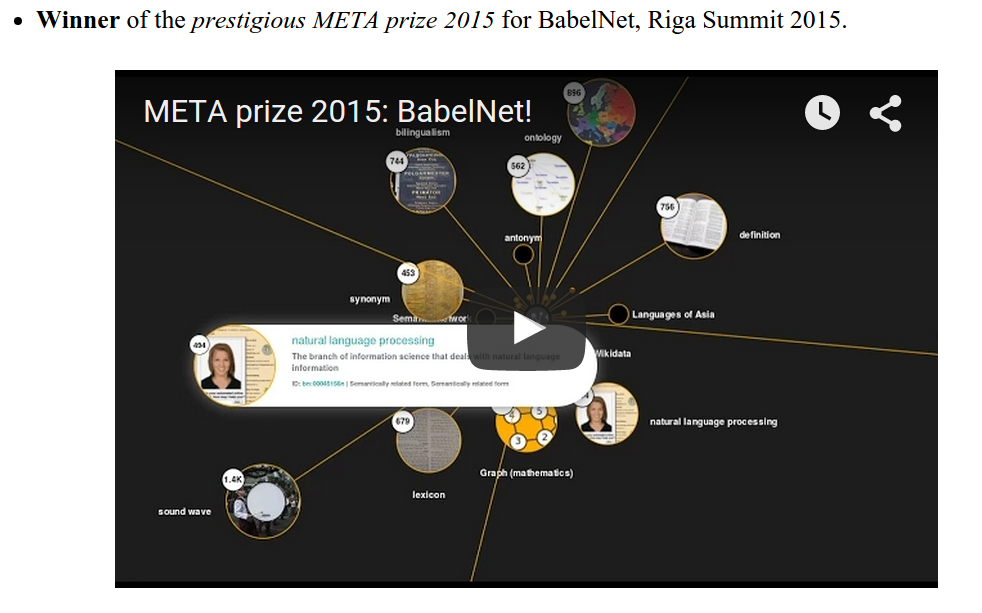
\includegraphics[width=0.6\hsize]{pic/navigli-babelNet.png}} 
	}}
      \end{overpic}
  \end{figure}

  \begin{columns}
   \column{0.55\hsize}
   \begin{block}{Claudio Delli Bovi}
    罗马大学博士,计算语言学方向,主要研究语法、句法结构,目前在做WSD
   \end{block}
   \column{0.4\hsize}
   \begin{block}{Luis Espinosa-Anke}
    庞培法布拉大学博士,在做一些信息抽取,语义网有关的东西
   \end{block}
  \end{columns}
   \begin{block}{Roberto Navigli}
    Claudio的导师,07年博士毕业,\textbf{BabelNet/Babelfy}
   \end{block}


}


\frame{
  \begin{columns}[c]
   \column{.15\hsize}
   \column{.7\hsize}
   \begin{block}{}
    \centering \Large 概述 \\ 
    \small --- 动机/方法简述
   \end{block}

   \column{.15\hsize}
  \end{columns}

}

\frame{
  \frametitle{\only<1-2>{summary/motivation}\only<3->{summary/method}}
  \begin{columns}
  \column{0.99\hsize}
      \begin{footnotesize}
  \begin{tikzpicture}
    \tikzstyle{Node}=[draw, rectangle, rounded corners, align=center]
    \node [Node, text width=2.5cm] (entity) {
      \emph{实体} \\ 
      \begin{footnotesize}
      \red{李娜(网球运动员)} \\ 
      \red{ 李娜(歌手)}\\
      \red{李娜(游泳运动员)}\\
      \red{姜山(网球运动员)}\\
      \red{张家辉 \\ ...}\\
      \end{footnotesize}
    };
%     \node [Node, text width=1.5cm, right=of entity] (type) {
%       \emph{关系} \\ 
%       \begin{footnotesize}
%       \brown{配偶}\\
%       \brown{出生日期}\\
%       \brown{子女\\ ...}\\
%       \end{footnotesize}
%     };
    \only<4>{
    \node [Node, text width=3cm, right=of entity] (exap1) {
      【一】\\
      \begin{footnotesize}
      \blue{微软-CEO-纳德拉}
      \blue{搜狐-CEO-张朝阳}\\
      \blue{\red{苹果(?)}-CEO-库克}\\
      ...
      \end{footnotesize}
    };
    }
    \only<5>{
    \node [Node, text width=3cm, right=of entity] (exap1) {
      【二】\\
      \begin{footnotesize}
      \blue{花果山-所在-连云港}\\ 
      \blue{全国政协-所在-北京}\\ 
      \blue{\red{大众}-所在-黑龙江} (这里指大众乡)
      ...
      \end{footnotesize}
    };
    }
    \node [Node, text width=3.5cm, below=of entity] (tripleWP) {
      zh.baidubaike:李娜-丈夫-姜山
    };
    \node [Node, text width=4cm, below=of tripleWP] (tripleNew) {
      \begin{footnotesize}
      \red{李娜(网球运动员)}-\brown{配偶}-\red{姜山}
      \end{footnotesize}
    };
    \node [Node, text width=3.5cm, below=of tripleNew] (tripleHD) {
      zh.hudong:李娜(网球)-夫婿-姜山(湖北人)
    };
    \node [Node, text width=7.05cm, right=of tripleNew] (desc) {
   \only<1>{
    \begin{large}
     如何整合多个知识库?\\
    \end{large}
    假设
    \begin{itemize}\begin{footnotesize}
     \item 全部在subject-predicate-object数据库上
     \item 知识库可能是完全非结构化的(主语只是普通字符串)
     \item 给定一个完备的语义集合(左上的实体集合)
     \item 其他的数据库可能存在歧义,结构不标准
     \end{footnotesize}
    \end{itemize}

   }
   \only<2>{
    \begin{large}
     如何整合多个知识库?\\ 
    \end{large}
    过程
    \begin{itemize}\begin{footnotesize}
     \item 怎么把\blue{李娜-丈夫-姜山}转换成标准的结构?
     \item 消歧+谓词统一
      \begin{itemize}
       \item 消除其他数据库中主体、客体的歧义
       \item 将不同数据库中含义相同的谓词合并
      \end{itemize}
     \end{footnotesize}
    \end{itemize}
  }
  \only<3->{
    \begin{large}
     如何整合多个知识库?\\
    \end{large}
    方法
      \begin{itemize}
  \only<3>{
    \begin{footnotesize}
     \item 先对\red{\textbf{实体消歧}},再对应不同数据库的\red{\textbf{relation归一}}
     \item \red{\textbf{实体消歧}}【1】
      \begin{itemize}\begin{footnotesize}
       \item 对一条三元组的主体、客体的语义候选的所有组合,如果存在一组\red{已经非常好}了,选为\red{种子}
     \item 找出好的relation (主体的向量集中,比如都表示人;客体的向量集中,比如都表示地点)
       %\item 计算每种relation的\red{种子三元组}中主体、客体的语义向量的均值作为该关系的\red{特征主语向量}、\red{特征客体向量}
       \end{footnotesize}
      \end{itemize}
%     \item \red{\textbf{实体消歧}}【2】
%     \begin{itemize}\begin{footnotesize}
%      \item 找出好的relation (主体的向量集中,比如都表示人;客体的向量集中,比如都表示地点)
%      \end{footnotesize}
%     \end{itemize}

     \end{footnotesize}
  }
  \only<4-6>{
    \begin{footnotesize}
      \only<4->{
    \item \red{\textbf{实体消歧}}【2】
      \begin{itemize}\begin{footnotesize}
       \item 【一】对于好的relation,该关系内的所有三元组的主体、客体相互间相似,可以作为其中一个主体做消歧时的文本
	\only<5->{
       \item 【二】对于不好的relation对应的一条三元组的主语或客体,只能通过relation名字来消歧
       }
       \end{footnotesize}
      \end{itemize}
	}

    \end{footnotesize}
  }
  \only<7>{
    \item 不同知识库的\red{\textbf{relation归一}}
    \item 通过每两个知识库的每任两个relation的\red{主客体特征向量}计算相似性
  }
  \end{itemize}
  }
    };
    \path[-Stealth, blue, thick] 
     (tripleWP) edge [bend left=10] (tripleNew)
     (tripleHD) edge [bend left=10] (tripleNew)
     ;
  \end{tikzpicture}
      \end{footnotesize}

  \end{columns}
}


\frame{
  \begin{columns}[c]
   \column{.15\hsize}
   \column{.7\hsize}
   \begin{block}{}
    \centering \Large 相关工作 \\ 
   \end{block}

   \column{.15\hsize}
  \end{columns}

}

\frame{
  \frametitle{related work/introduction}
  \begin{itemize}
   \item Open Information Extraction
    \begin{itemize}
     \item 从Web-scale级别的自然语言信息中抽取结构化/格式化的数据
      \begin{itemize}\begin{footnotesize}
       \item e.g. DBpedia, Freebase, YAGO,...
       \end{footnotesize}
      \end{itemize}

     \item 提升效果/去除噪声数据的方法
      \begin{itemize}
       \item matrix factorization, distant supervision, multi-instance,...
      \end{itemize}
     \item 知识库补全(Knowledge Base completion)
      \begin{itemize}
       \item 少量结构化数据和大量的半结构化数据相互提升准确率
      \end{itemize}
    \end{itemize}

  \end{itemize}

}

\frame{
  \frametitle{related work}
  \begin{itemize}
   \item BabelNet
    \begin{itemize}
     \item 罗马大学开发的跨语言语义网,\begin{footnotesize}以“姚明”为例\end{footnotesize}
      \begin{itemize}
       \item “entity”都是实体,有中文标签;“relation”纯英文
       \item “relation”有重复,无意义的
      \end{itemize}
    \end{itemize}
  \end{itemize}
    \begin{center}
     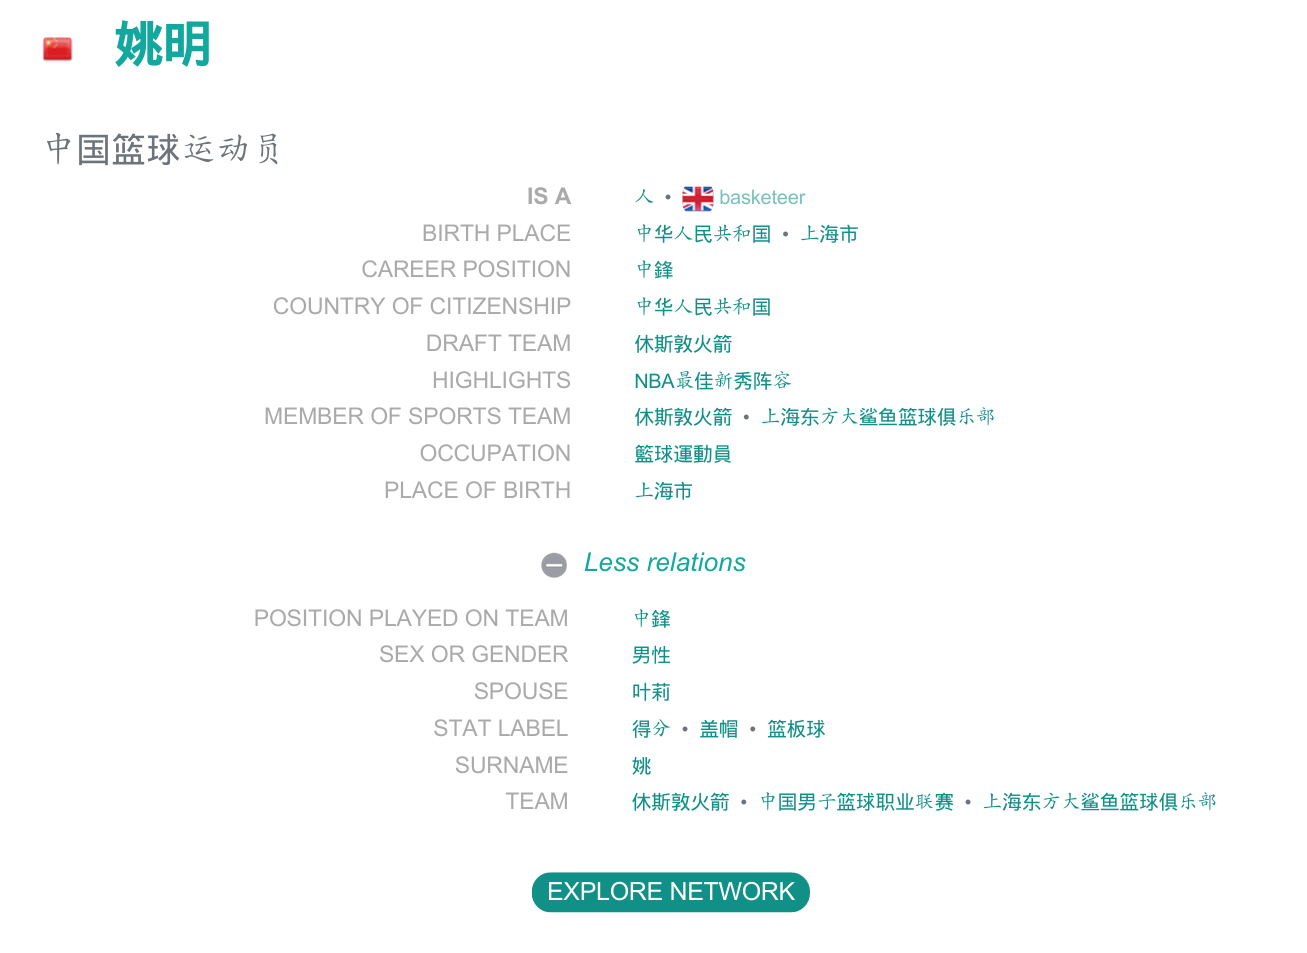
\includegraphics[width=0.7\hsize]{pic/babelNet.png}
    \end{center}

}

\frame{
  \frametitle{related work}
  \begin{itemize}
   \item Babelfy
    \begin{itemize}
     \item 罗马大学开发的多语言的消歧和实体链接集成的工具
      \begin{itemize}
       \item 链接到BabelNet
       \item 分词效果不好;
       \item 有一定的消歧能力:能找出网球运动员李娜,找不到歌手李娜
      \end{itemize}

    \end{itemize}

  \end{itemize}
    \begin{center}
     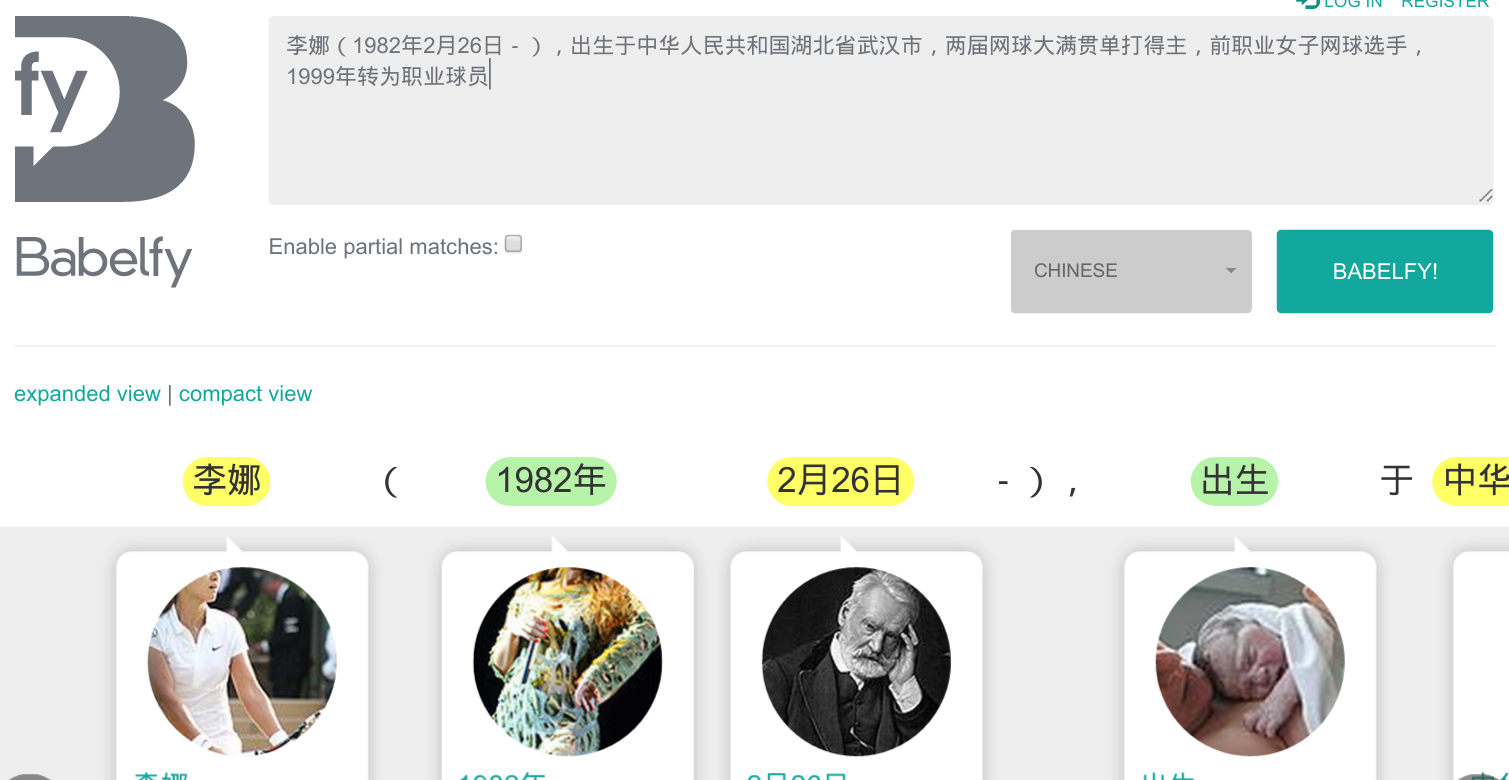
\includegraphics[width=0.8\hsize]{pic/babelfy.png}
    \end{center}

}

\frame{
  \frametitle{related work}
  两个数据库间的归一/对应
  \begin{block}{}
   \begin{itemize}
    \item  Dutta et al. (2014): \begin{footnotesize}NELL 数据集的 augment 链接到 DBpedia的实体 \end{footnotesize}
      \begin{itemize}
       \item 使用一阶逻辑和马尔可夫网络
      \end{itemize}
   \end{itemize}
  \end{block}

  \begin{block}{}
   \begin{itemize}
    \item Grycner and Weikum (2014) :\begin{footnotesize}PATTY的pattern 和 wordNet的谓词 对应\end{footnotesize}
   \end{itemize}
  \end{block}

  \begin{block}{}
   \begin{itemize}
    \item Lin et al. (2012) :\begin{footnotesize}使用freebase的类别来链接reverb中的潜在实体\end{footnotesize}
      \begin{itemize}
       \item reverb record:[2047542	\red{Bilberry}	also\_contains	\red{vitamin\_C}	bilberry	also\_contain	vitamin\_c	1	0.94124	http:...]
      \end{itemize}
   \end{itemize}
  \end{block}
  
}

\frame{
  \frametitle{related work}
  能适应多个数据库归一的方法
  \begin{block}{}
   \begin{itemize}
    \item Riedel et al. (2013):\begin{footnotesize}训练含有隐式特征(latent feature)的实体向量、关系向量\end{footnotesize}
   \end{itemize}
  \end{block}

  \begin{block}{}
   \begin{itemize}
    \item Dong et al. (2014):\begin{footnotesize}使用freebase数据训练一个概率模型来判断抽取结果的准确度\end{footnotesize}
   \end{itemize}

  \end{block}
  在关系抽取和知识补全上使用Embedding models
  \begin{block}{}
    \begin{itemize}
     \item Socher et al., 2013; Weston et al.,2013; Bordes et al., 2013
    \end{itemize}
  \end{block}
    \begin{itemize}
     \item 作者认为这些模型停留在(surface level),不能表达普世的语义(common semantic)\only<2>{\red{【不能区分多义词?】}}
    \end{itemize}

}


\frame{
  \begin{columns}[c]
   \column{.15\hsize}
   \column{.7\hsize}
   \begin{block}{}
    \centering \Large 归一化方法 \\ 
    \small --- 实体消歧
   \end{block}

   \column{.15\hsize}
  \end{columns}

}

\frame{
  \frametitle{method/disambiguation}
  \begin{columns}
   \column{0.35\hsize}
   \begin{footnotesize}
  \begin{tikzpicture}
    \tikzstyle{Node}=[draw, rectangle, rounded corners, align=center]
    \node [Node, text width=2.5cm] (entity) {
      \emph{BabelNet实体} \\ 
      \begin{footnotesize}
      \red{李娜(网球运动员)} \\ 
      \red{ 李娜(歌手)}\\
      \red{李娜(游泳运动员)}\\
      \red{姜山(网球运动员)}\\
      \red{张家辉 \\ ...}\\
      \end{footnotesize}
    };
    \node [Node, text width=3.5cm, below=of entity] (tripleWP) {
      zh.wikipedia:李娜-丈夫-姜山
    };
    \node [Node, text width=4cm, below=of tripleWP] (tripleNew) {
      \begin{footnotesize}
      \red{李娜(网球运动员)}-丈夫-\red{姜山}
      \end{footnotesize}
    };
    \path[-Stealth, blue, thick] 
     (tripleWP) edge [bend left=10] (tripleNew)
     ;
  \end{tikzpicture}
  \end{footnotesize}
  
  \column{0.6\hsize}
  \only<1-4>{
    【实体消歧】准备
  \begin{itemize}
   \item BabelNet是一个语义集合(sense inventory),与常见知识库的实体对应
   \item 消歧结束
    \begin{itemize}
     \item 知识库的主语/客体对应到BabelNet上
    \end{itemize}

   \item 实体/语义向量
    \begin{itemize}\begin{footnotesize}
     \item 利用一个庞大的标注语料训练词向量
     \item 采用SENSEMBED(罗马大学2015ACL)训练而非word2vec,因为后者不能区分多义词
     \end{footnotesize}
    \end{itemize}
     \only<2>{
      \begin{block}{}\begin{footnotesize}
       按照论文的图,作者是拿维基百科训练的。\\ 
       而维基百科内部链接做的很好,很多地方被人工消歧了。\\ 
       可以训练出多个词向量\{苹果、蘋果公司\}?
       \end{footnotesize}
      \end{block}
     }
     \only<3>{
     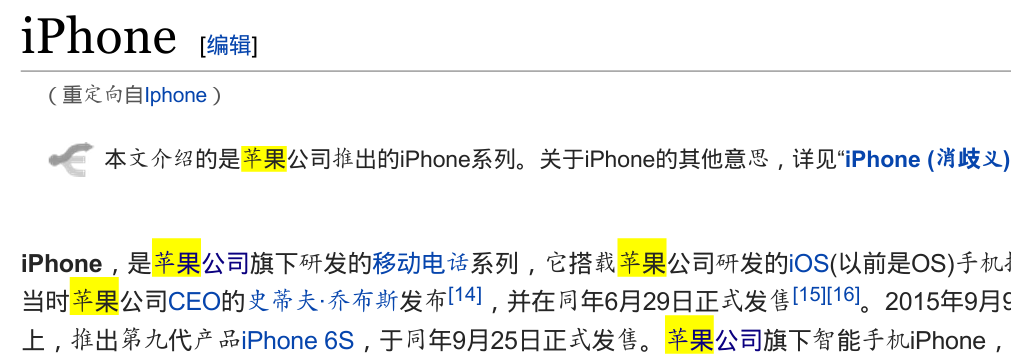
\includegraphics[width=0.9\hsize]{pic/wikiWSD.png}
     }
    \end{itemize}
   }
   \only<5-7>{
    【实体消歧一】找出\red{种子三元组}
    \begin{itemize}
     \item 三元组<$e_d,r,e_g$>,$e_d,e_g$的所有语义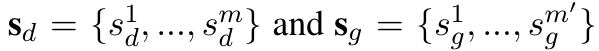
\includegraphics[width=0.6\hsize]{pic/sdsg.png},
      对应的词向量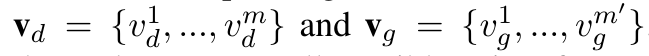
\includegraphics[width=0.6\hsize]{pic/vdvg.png}
     \item 任意两个组合中词向量余弦相似度最大的一对作为该三元组消歧的默认最优解
      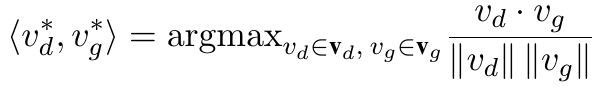
\includegraphics[width=0.6\hsize]{pic/sdsg2.png}
     \item 如果最优解的相似度大于一个阈值$\zeta$,那么这个最有解是“完美”的,该三元组即为\red{种子三元组}
     \only<6>{
      \begin{block}{}
      \begin{itemize}\begin{footnotesize}
       \item 关系$r$的三元组的主语、客体的词向量可能是满足一个特定的“角度”才是标注的?
       \end{footnotesize}
      \end{itemize}
      \end{block}
      }
    \end{itemize}
   }
   
   \only<8>{
    【实体消歧二】找出\red{完美关系}
    \begin{block}{def.完美关系}\begin{footnotesize}
     该relation对应的主语(客体)的词向量很集中,方差小
     \end{footnotesize}
    \end{block}

    %对于关系r
    \begin{itemize}\begin{footnotesize}
     \item $v_D,v_G$表示关系r对应的所有\red{种子三元组}的主语、客体的词向量集合
     \item 该关系的主语、客体中心词向量为 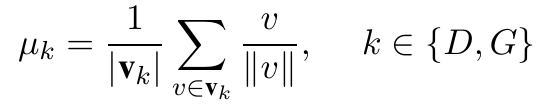
\includegraphics[width=0.6\hsize]{pic/uk.png}
     \item 该关系的主语、客体方差为\\ 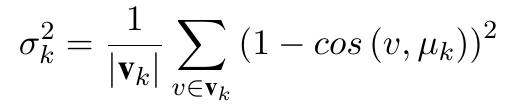
\includegraphics[width=0.6\hsize]{pic/sitak.png}
     \item 该关系的总体方差为主客体方差的平均数
     \item 方差越小,说明该关系对应的种子三元组越好
     \item 如果总体方差小于某个阈值$\delta$,则认为其是\red{完美关系}
     \end{footnotesize}	
    \end{itemize}
   }
   
   \only<9>{
    【实体消歧三】实体消歧(分类)
    对于任意一个三元组<$e_d,r,e_g$>,比如想要判断$e_d$的含义
    \begin{itemize}
     \item 如果$r$是好的关系
    \begin{block}{}\begin{footnotesize}
     那么$r$内的种子三元组能正确的反应$r$的含义,使用种子三元组的主语可以作为$e_d$消歧的依据
     \end{footnotesize}
    \end{block}
     \item 如果$r$不是好的关系
    \begin{block}{}\begin{footnotesize}
     只用当前这条三元组的$r,e_g$来作为$e_d$分类/消歧的依据
     \end{footnotesize}
    \end{block}
    \end{itemize}

   }

  \end{columns}

}

\frame{
  \begin{columns}[c]
   \column{.15\hsize}
   \column{.7\hsize}
   \begin{block}{}
    \centering \Large 归一化方法 \\ 
    \small --- 关系(relation)归一
   \end{block}

   \column{.15\hsize}
  \end{columns}

}

\frame{
  \frametitle{method/unification}
  和 disambiguation 过程类似
  \begin{enumerate}
   \item 对于每个知识库的每种关系,计算其主体、客体的平均向量
   \item 对于任意两个知识库的任意关系对$r_i,r_j$,其相似性为$(s_D+s_G)/2$ 
    \begin{itemize}
     \item $s_k$定义如下,$k\in\{D,G\}$,其中$\mu_{D}^{r_j}$表示关系${r_j}$的主语向量的平均值
    \end{itemize}


  \end{enumerate}
  \begin{center}
   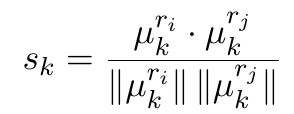
\includegraphics[width=0.35\hsize]{pic/sk.png}
  \end{center}


}

\frame{
  \begin{columns}[c]
   \column{.15\hsize}
   \column{.7\hsize}
   \begin{block}{}
    \centering \Large 实验 \\ 
   \end{block}

   \column{.15\hsize}
  \end{columns}

}

\frame{
  \frametitle{experiment}
  【数据集】4个,后两个内部有链接(linked resources),前两个没有
  \begin{center}
     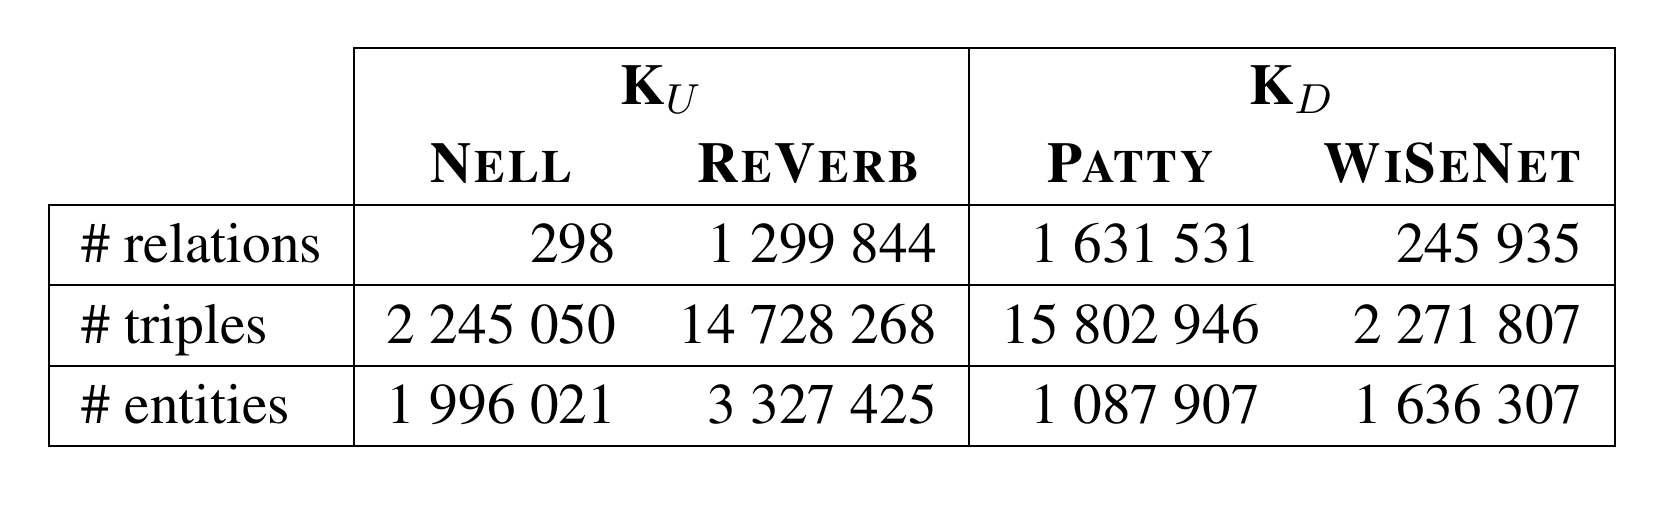
\includegraphics[width=0.5\hsize]{pic/ds.png}
  \end{center}

  【额外实验】测试\red{种子三元组}的正确率
    \begin{itemize}\begin{footnotesize}
     \item 实验的时候认为\red{种子三元组}是完全正确的,实际有一点错误
     \item 测试在patty上:左边是在全部种子三元组的情况,右边是去掉本来就无歧义的种子三元组
     \end{footnotesize}
    \end{itemize}
    \begin{center}
     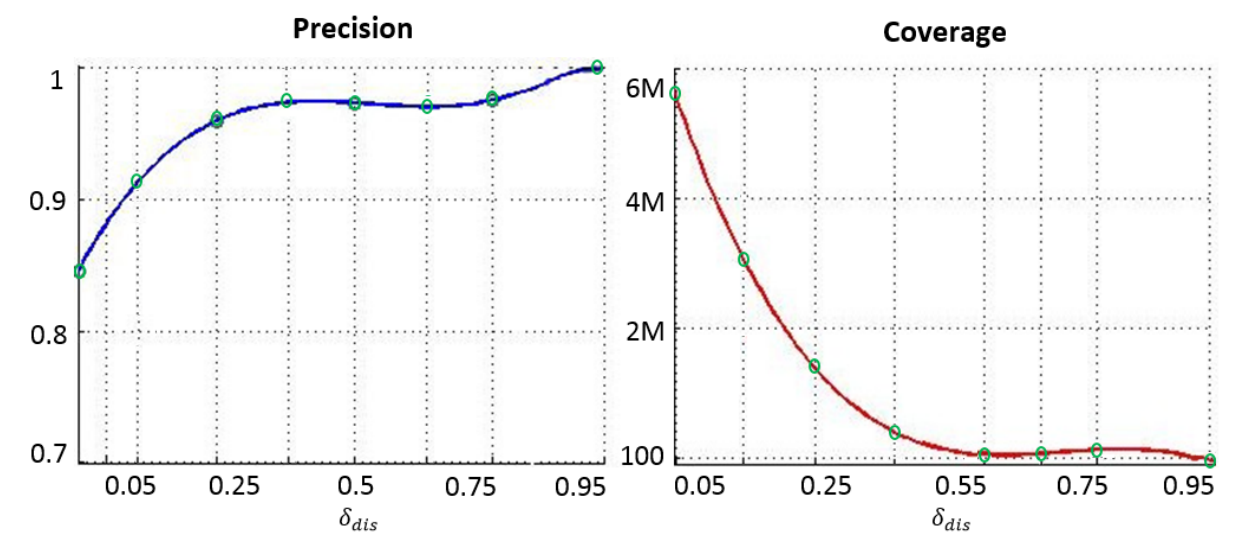
\includegraphics[width=0.5\hsize]{pic/seedCover.png}
     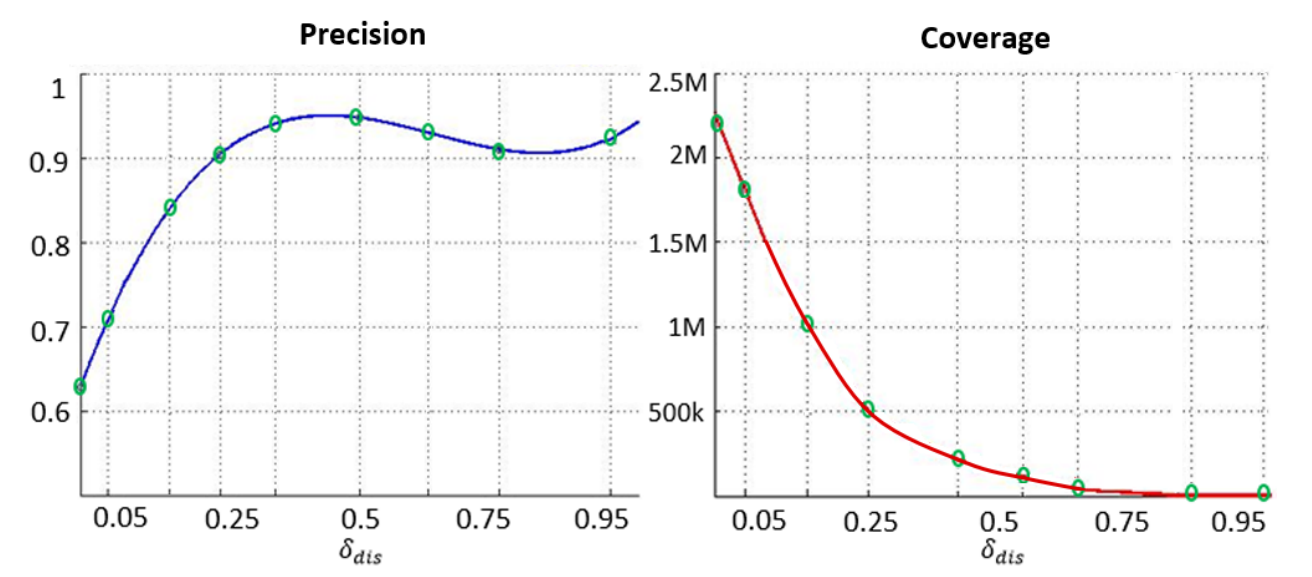
\includegraphics[width=0.5\hsize]{pic/seedCoverSubset.png}
%      \begin{overpic}[scale=.15]
% 	{pic/seedCover.png}
% 	\only<2>{\put(0,0){
% 	  \setlength{\fboxrule}{0pt} 
% % 	  \setlength{\fboxsep}{-7.5cm} 
% 	  \fbox{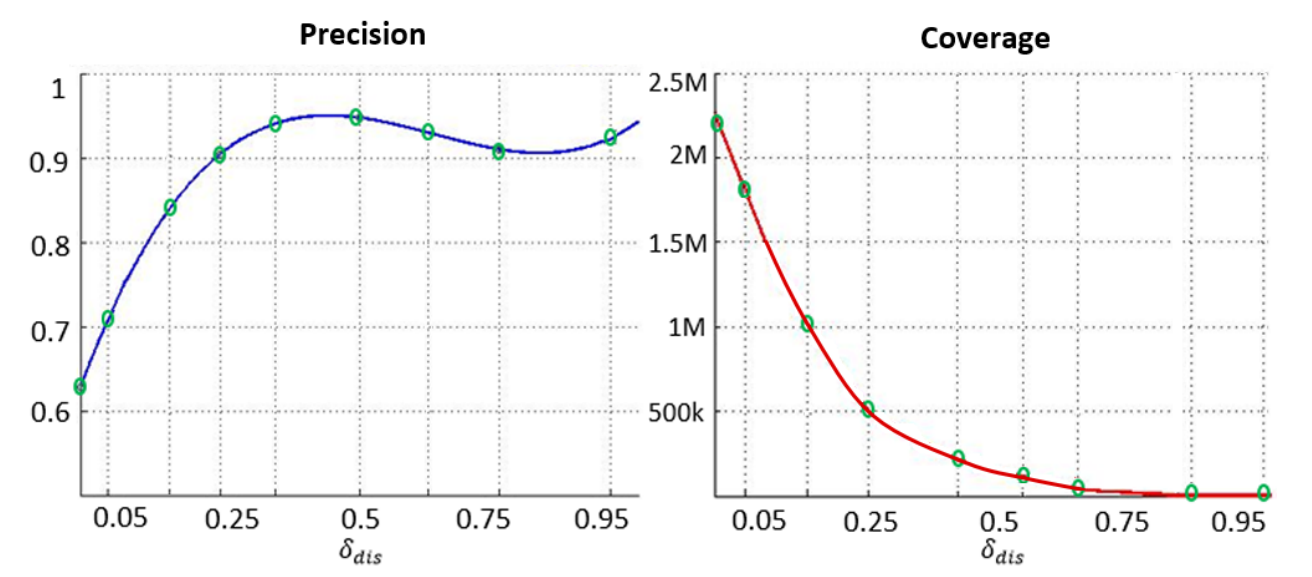
\includegraphics[width=0.5\hsize]{pic/seedCoverSubset.png}} 
% 	}}
%       \end{overpic}
    \end{center}
}

\frame{
  \frametitle{experiment}
  【主要实验一】测试消歧准确率
    \begin{itemize}
     \item 上图的Baseline是指不选seed
      \begin{itemize}
       \item 任意一个词消歧时只把他所在的那条三元组的主语、客体、谓词作为上下文消歧,和该关系的其他三元组无关
       \item $\zeta$越大表示种子三元组越准确,准确率会更高
      \end{itemize}
    \end{itemize}
    \begin{center}
     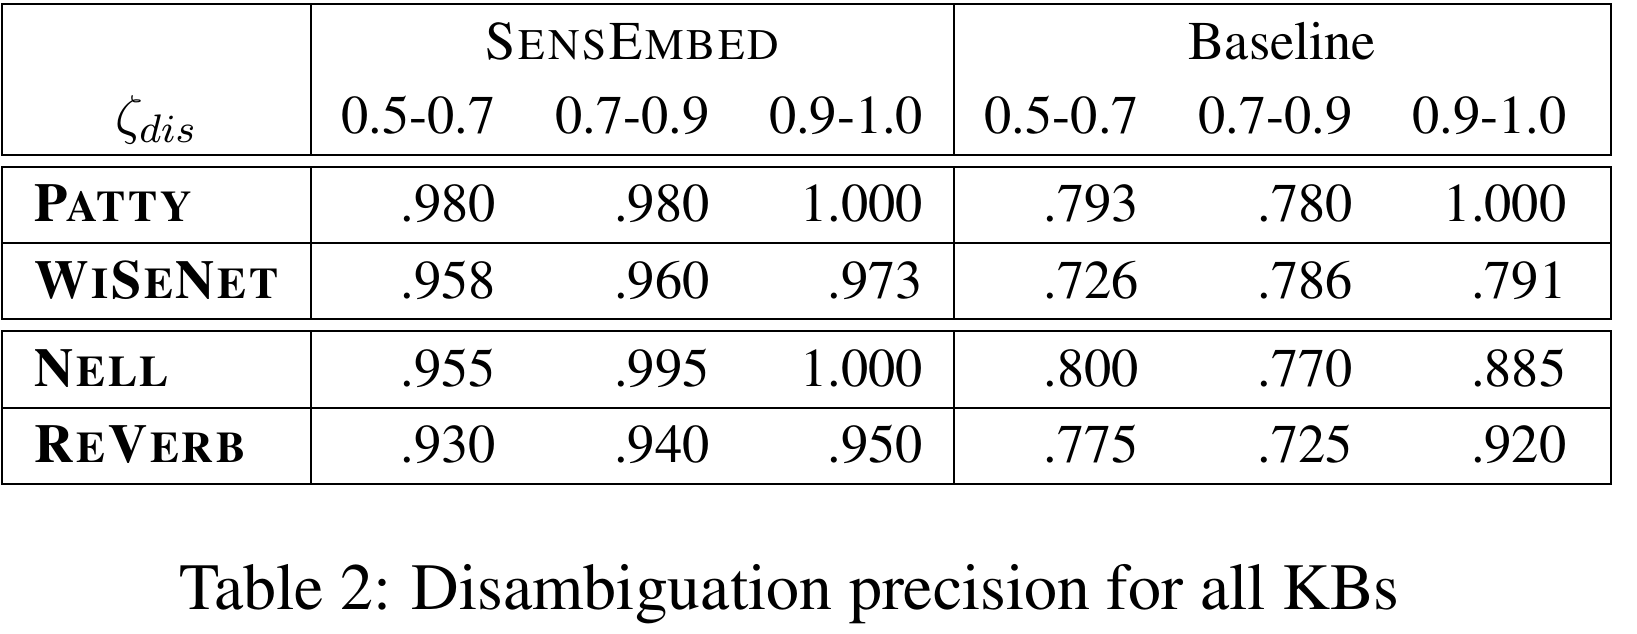
\includegraphics[width=0.7\hsize]{pic/dp.png}
    \end{center}
}
\frame{
  \frametitle{experiment}
  【主要实验一】测试消歧准确率
    \begin{itemize}

     \item 下图的“only seed”是指只采用每个类别的种子三元组来表示给类别的主语、客体,进而预测三元组的主语、客体的类别
      \begin{itemize}
       \item 不论是否“完美”,都按“完美”考虑
      \end{itemize}
     \item (?)PATTY和WISENET本身对应到维基百科实体,理论不用消歧,准确率是100\%:可能是因为:
      \begin{itemize}
       \item 一些维基百科本身对应错误
       \item 作者的方法其实也可以使用在已链接的主客体上
      \end{itemize}


      %\item 类似于”随大溜“,多数投票
    \end{itemize}
    \begin{center}
     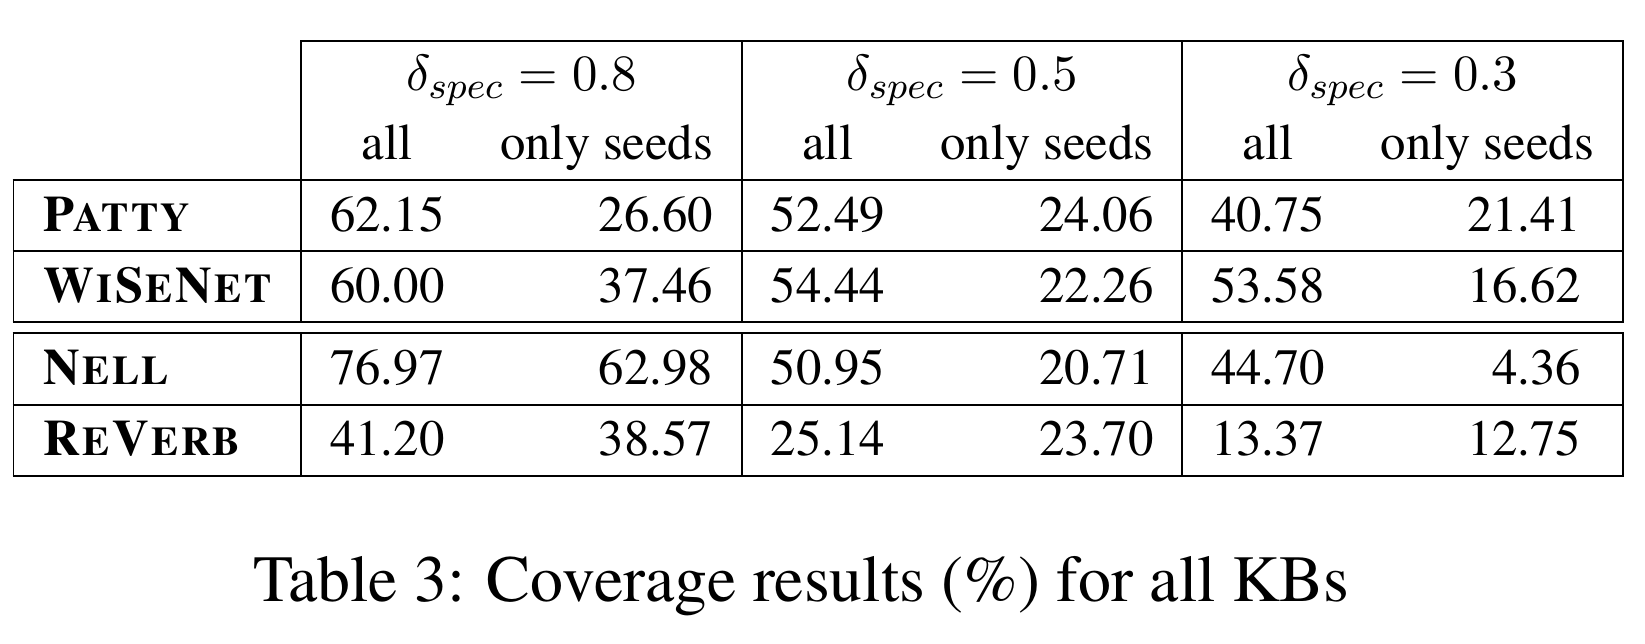
\includegraphics[width=0.7\hsize]{pic/cr.png}
    \end{center}
}


\frame{
  \frametitle{experiment}

  【额外实验二】不同relation对主客体的限制
  \only<1>{
   \begin{columns}
    \column{0.6\hsize}
    \begin{center}
     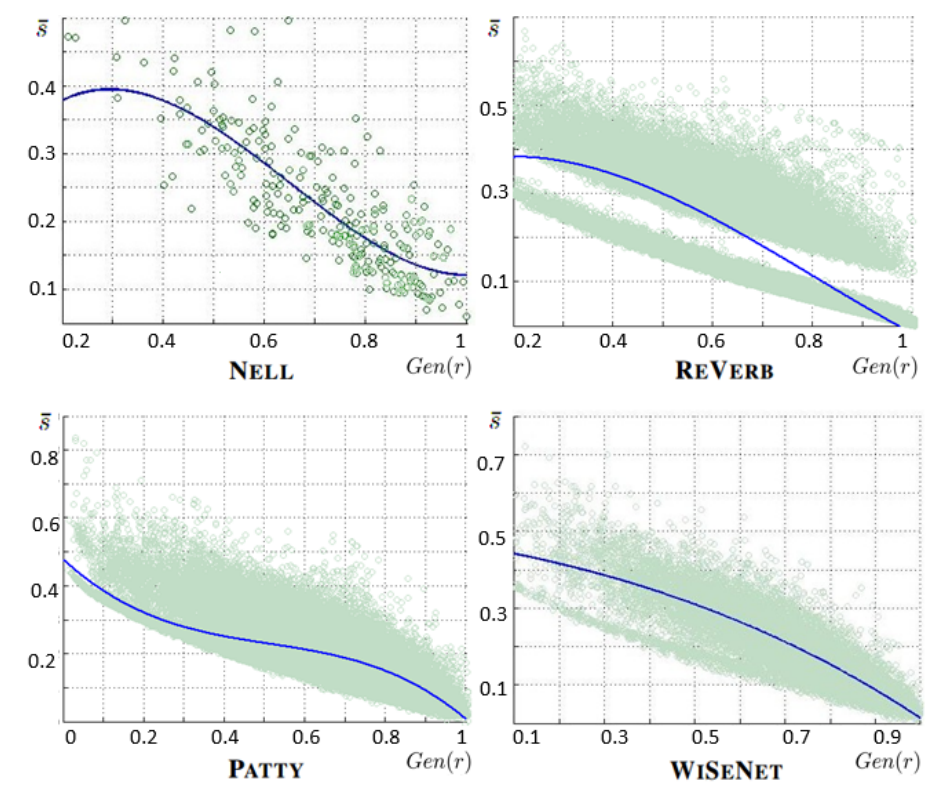
\includegraphics[width=0.95\hsize]{pic/relationCons.png}
    \end{center}
    \column{0.4\hsize}
    \begin{itemize}\begin{footnotesize}
     \item $Gen(r)=(\sigma_{D}+\sigma_{G})/2$\\ (主客体的方差)的均值
     \item $\bar s=avg_{v_r=r}(v_d*v_g)$\\ (三元组的主客体相似度)的均值
     \item $Gen(r)$ 越大说明relation要求越严格
     \item $\bar s$ 越大说明主客体的类别要求越低(都是随机出现,则$\bar{s}\approx\sqrt{2}/2\approx 0.7$?)
     \item \textbf{越普适的relation,对主客体的要求越低}
     \end{footnotesize}
    \end{itemize}
   \end{columns}
   }
   \only<2>{
   \begin{columns}
    \column{0.6\hsize}
    \begin{center}
     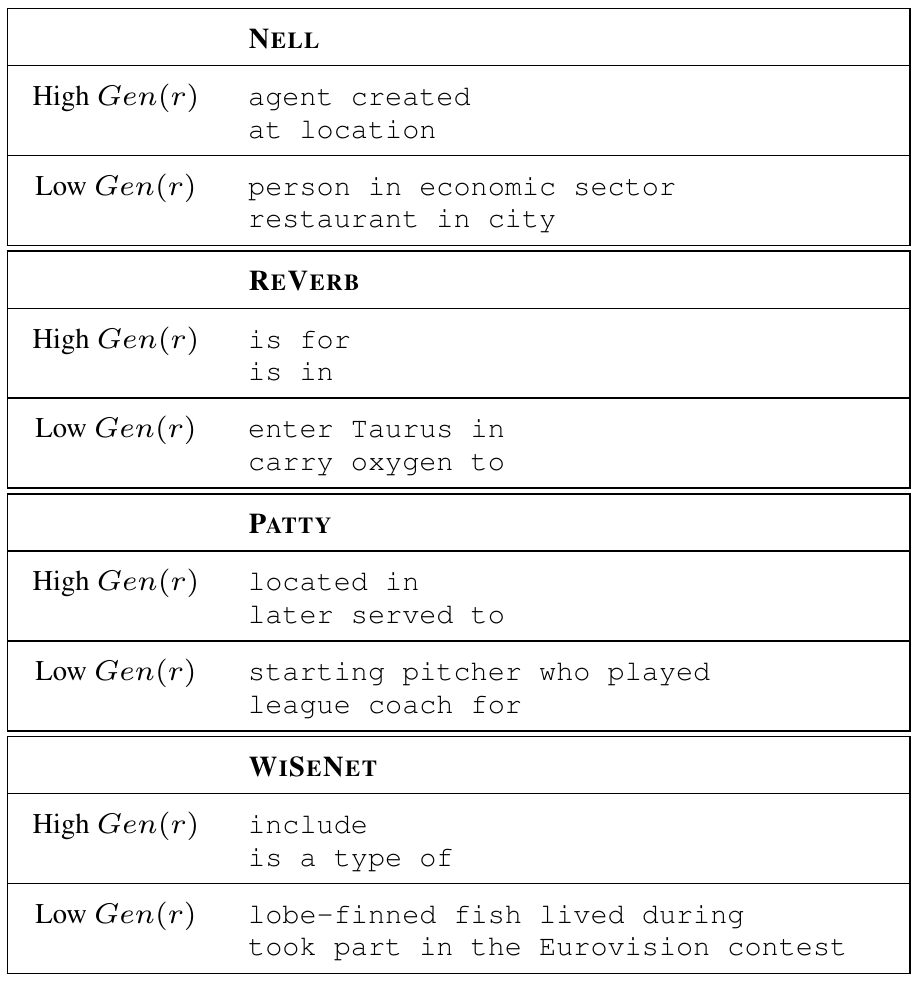
\includegraphics[width=0.8\hsize]{pic/relationExp.png}
    \end{center}
    \column{0.4\hsize}
    \begin{itemize}
     \item 例子
    \end{itemize}
   \end{columns}
   }
}

\frame{
  \frametitle{experiment}
  【主要实验二】测试relation对应的准确率
  \only<1>{
  \begin{itemize}
   \item 为了方便测试,每个数据集只取前1w个关系,相互对应
    \begin{itemize}
     \item 随机选取150对,人工判定
    \end{itemize}
  \end{itemize}
    \begin{center}
     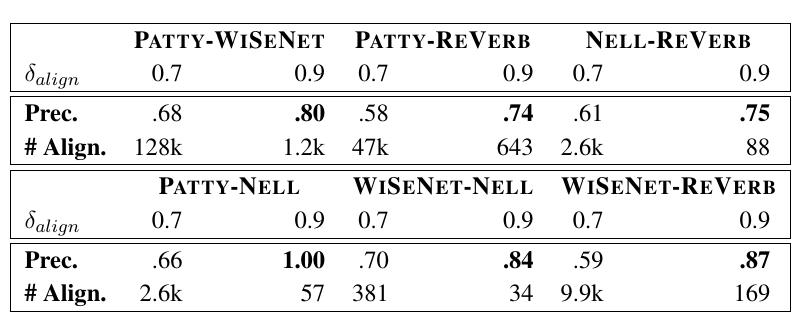
\includegraphics[width=0.7\hsize]{pic/ca.png}
    \end{center}
    }
   \only<2>{
  \begin{itemize}
   \item 对齐的样例
  \end{itemize}
    \begin{center}
     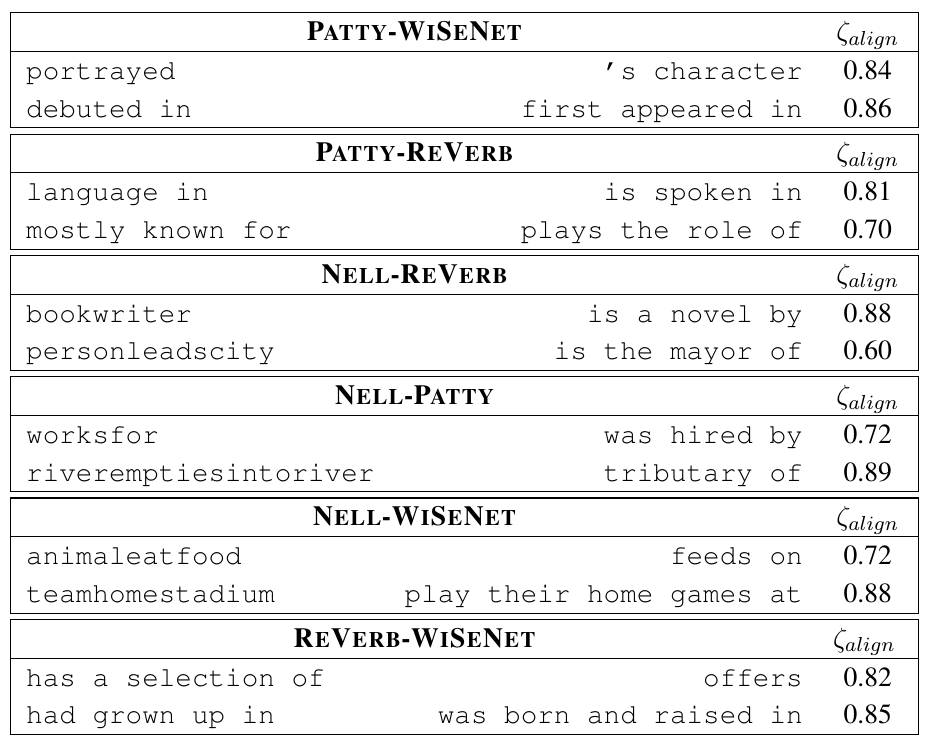
\includegraphics[width=0.5\hsize]{pic/alignExap.png}
    \end{center}
    }
   
}


\frame{
  \begin{columns}[c]
   \column{.15\hsize}
   \column{.7\hsize}
   \begin{block}{}
    \centering \Large 总结 \\ 
   \end{block}

   \column{.15\hsize}
  \end{columns}

}

\frame{
  \frametitle{conclusion}
  \begin{itemize}
   \item 出发点
  \begin{itemize}
   \item 同一个关系的不同实例应该有相似的词向量,主语互相比较相像,客体也是
   \item 不同知识库如果使用同一套主语、客体entity,那么不同知识库之间的相同关系应该有相似的主语、客体形式
  \end{itemize}

   \item 实验效果
  \begin{itemize}
   \item 对\red{种子三元组}和\red{完美关系}这两处筛选/排序使得好的数据起到更大的作用
   \item (缺点)没有统一的评价体系,相互间的优劣不能对比:“我们和别的系统不同;不能照搬;无法比较效果”,很多手工筛选检查
  \end{itemize}
  \end{itemize}

}

\frame{
  \begin{center}
   \Large 问题?
  \end{center}

}

\end{document}

